\documentclass[prb,9pt,notitlepage]{revtex4-1}
%\documentclass[a4paper,twocolumn,9pt]{article}

%\usepackage{geometry}
%\geometry{a4paper,top=2.5cm,bottom=2cm,inner=1.5cm,outer=1.5cm}

\usepackage{mwe}% just for the example content
\usepackage{color}
\usepackage{latexsym,amsmath}
\usepackage{physics}
\usepackage{listings}
\usepackage[dvipsnames]{xcolor}
\usepackage{parskip}
\usepackage{hyperref}
%\usepackage{dblfloatfix}
%\usepackage{subfig}
\definecolor{linkcolor}{rgb}{0,0,0.65}%hyperlink
\definecolor{shadecolor}{rgb}{0.93, 0.93, 0.93}
%\usepackage[pdftex,colorlinks=true, pdfstartview=FitV, linkcolor= linkcolor, citecolor= linkcolor, urlcolor= linkcolor, hyperindex=true,hyperfigures=true]{hyperref} %hyperlink%
%\usepackage[backend=biber, sorting=ynt]{biblatex}
%\usepackage{ragged2e} % to justify caption
%\addbibresource{bibliography.bib}
 \usepackage{booktabs}

\usepackage[T1]{fontenc}
\usepackage{xcolor}
\usepackage{lmodern}
\usepackage{listings}
\lstset{language=[95]Fortran,
  backgroundcolor=\color{shadecolor},
  basicstyle=\ttfamily,
  keywordstyle=\color{blue},
  commentstyle=\color{gray},
  stringstyle=\color{red},
  showstringspaces=false
  %morecomment=[l]{!\ }% Comment only with space after !
}

\usepackage{tabularx}

\usepackage{fancyhdr}
\pagestyle{fancyplain}% <- use fancyplain instead fancy
\fancyhf{}
\fancyhead[R]{\today}
\fancyhead[L]{Alessandro Lambertini}
\fancyfoot[L]{Quantum information and computing}
\fancyfoot[C]{Report 2}
\fancyfoot[R]{\thepage}

\renewcommand{\headrulewidth}{0pt}

\usepackage{float}
\usepackage{siunitx}




\begin{document}
\title{Quantum information and computing: Exercises report, week 4. \\ Multi-run script \& Automated fits }

\author{Alessandro Lambertini}


\date{\today}

\begin{abstract}
Through the exercise of this week, we try to numerically describe the time evolution of a 1-D quantum harmonic oscillator by solving the eigenvalues problem exploiting the subroutines written for the previous exercises and applying the Split Operator Method to numerically approximate the time evolution operator. In particular, we are requested to compute the time evolution for the ground state of the quantum harmonic oscillator for different time $t$.
\end{abstract}

\maketitle

\section{Theory}
We aim to solve the problem of finding the evolved state $\ket{\psi(t=T)}$ of a quantum harmonic oscillator, given the boundary condition $\ket{\psi(t=0)}=\ket{\psi_0}$, according to the time-dependent Schroedinger equation:
\begin{equation}
  i\hbar \frac{\partial \ket{\psi}}{\partial t} = \hat{H}\ket{\psi} \qquad \mbox{where} \qquad H = \hat{p}^2/2 + \frac{(\hat{q}-q_0(t))^2}{2} \quad ; \quad q_0(t) = \frac{t}{T} \quad ; \quad t \in [0;T]
\end{equation}
The split operator method stems from the observation that the two parts of the Hamiltonian being functions of a single variable, either $\hat{x}$ or $\hat{p}$, are diagonal in the space and momentum representation respectively. Therefore, we can exploit the Baker-Campbell-Hausdorff formula and split the operator even if the two parts don't commute, given a sufficiently small $\Delta t$, in the following way:
\begin{equation}
  	e^{-\frac{i}{\hbar}\hat{H}(t) \Delta t} = e^{-\frac{i}{\hbar}\frac{\hat{V}(x,t)}{2} \Delta t} e^{-\frac{i}{\hbar} \hat{T} \Delta t}  e^{-\frac{i}{\hbar}\frac{\hat{V}(x,t)}{2} \Delta t} +\mathcal{O}(\Delta t^3) \label{som}
\end{equation}
With the approximation in \ref{som} we can exploit the Fourier transform, possibly the fast one, to run from position space to momentum space and vice-versa and applying the different operators in their diagonal form.

\section{Code development}
In order to accomlish the tasks proposed by this exercise we exploit an extended version of the program implemented last week. Therefore, after having computed the ground state of the q.a.o. I decided to write a subroutine that implements the split operator method given the potential of the exercise:
\begin{equation}
	H=\frac{p^2}{2m}+\frac{1}{2} m \omega^2 \left(x-\frac{t}{T}\right)^2
\end{equation}

\begin{lstlisting}
!!!!!!!!!!!!!!!!!!!!! Temporal evolution !!!!!!!!!!!!!!!!!!!!
subroutine temporal_evolution(psi, t_max, t_resolution,&
 x_grid, omega, mass, h_bar, psi_evol)
  !declaration
  complex(kind=8), dimension(:,:), allocatable :: psi_evol
  complex(kind=8) :: psi(:)
  integer(kind=8) :: t_resolution, plan_forward, plan_backward, ii, jj
  real(kind=8) :: t_max, x_grid(:), t_grid(t_resolution),&
   delta_t, delta_x, omega, mass, h_bar, area

  allocate(psi_evol(size(x_grid),t_resolution+1))

  !time grid initialization
  delta_t = t_max/real(t_resolution-1,8)
  delta_x = 2*maxval(x_grid)/real(size(x_grid),8)

  psi_evol(:,1) = psi
  do ii=1,t_resolution
    t_grid(ii) = 0+(ii-1)*delta_t
  end do

  !prepare the system for the fourier transform
  call dfftw_plan_dft_1d(plan_forward,size(x_grid),psi,psi,-1,64);
  call dfftw_plan_dft_1d(plan_backward,size(x_grid),psi,psi,1,64);


  psi_evol(:,1) = psi
  do ii = 1,t_resolution

    !propagate the first half of the potential
    do jj = 1, size(x_grid)
      psi(jj) = psi(jj) * exp(cmplx(0,-delta_t/2*0.5*mass*omega**2/h_bar)*&
      (x_grid(jj)-t_grid(ii)/t_max)**2)
    end do

    !momentum space
    call dfftw_execute_dft(plan_forward,psi,psi)
    !propagate the kinetic term

    do jj=0, size(x_grid)/2-1
      psi(jj+1)=psi(jj+1)*exp(cmplx(0, -0.5*delta_t*4*acos(-1.0)**2/&
      (h_bar*mass*(delta_x*size(x_grid))**2))*jj**2)
    end do

    do jj=size(x_grid)/2, size(x_grid)-1
      psi(jj+1)=psi(jj+1)*exp(cmplx(0, -0.5*delta_t*4*acos(-1.0)**2/&
      (h_bar*mass*(delta_x*size(x_grid))**2))*(size(x_grid)-jj)**2)
    end do

    !back to the position space
    call dfftw_execute_dft(plan_backward,psi,psi)

    !propagate the second half of the potential
    do jj = 1, size(x_grid)
      psi(jj) = psi(jj) * exp(cmplx(0,-delta_t/2*0.5*mass*omega**2/h_bar)*&
      (x_grid(jj)-t_grid(ii)/t_max)**2)
    end do

    !normalize the evolved state
    psi = psi/real(size(x_grid),8)

    !store the evolved state in a matrix
    psi_evol(:,ii+1) = psi
  end do
  call dfftw_destroy_plan(plan_forward)
  call dfftw_destroy_plan(plan_backward)
end subroutine temporal_evolution
!!!!!!!!!!!!!!!!!!!!!!!!!!!!!!!!!!!!!!!!!!!!!!!!!!!!!!!!!!!!!!!!!!!!!!!!
\end{lstlisting}
In this subroutine we first introduce a proper discretization in time, then exploit the \textit{fftw3} library to perform the fast Fourier transform. after having applied the proper operator to the state. We store the state in each time frame from $0$ to $T$ as columns in the matrix \textit{psi\_evol}, in this way we can take advantage of the subroutines written previously for writing data on files.

To properly show what is physical in the system we have to write the modulus squared of each evolved state:
\begin{lstlisting}
!!!!!!!!!!!!!!!!!!!! compute the squared modulus of the  !!!!!!!!!!!!!!!!!!!
!!!!!!!!!!!!!!!!!!!!!!!!! elements of a matrix  !!!!!!!!!!!!!!!!!!!!!!!!!!!
subroutine mod_squared_matrix(mm)
  complex(kind=8), dimension(:,:) :: mm
  integer(kind=8), dimension(2) :: dimm
  integer(kind=8) :: ii,jj

  dimm = shape(mm)

  do ii=1,dimm(1)
    do jj=1,dimm(2)
      mm(ii,jj) = mm(ii,jj)*conjg(mm(ii,jj))
    end do
  end do
end subroutine mod_squared_matrix
!!!!!!!!!!!!!!!!!!!!!!!!!!!!!!!!!!!!!!!!!!!!!!!!!!!!!!!!!!!!!!!!!!!!!!!!
\end{lstlisting}

Finally the entire program:
\begin{lstlisting}
program q_harm_osc
  use ex07module
  implicit none

  complex(kind=8), dimension(:,:), allocatable :: matrix, psi_evol
  complex(kind=8), dimension(:), allocatable :: psi
  real(kind=8), dimension(:), allocatable :: xx
  real(kind=8) :: Re_z, x_max,step,freq,mass,h_bar,t_max, area
  integer(kind=8) ::  ii, N, k_columns, k_entries, t_resolution
  double precision, dimension(:), allocatable :: eigv

  !set the parameters of the problem
  N=1000
  x_max = 5
  freq = 1
  mass = 0.5
  h_bar = 1
  step = 2*x_max/real(N-1,8)
  k_columns = 1001
  k_entries = 10
  t_max = 3
  t_resolution = 1000

  allocate(psi(N))

  !initialize the matrix and store it in a file
  call init_tridiag_qao_matrix(matrix, x_max,xx, N, freq, mass, h_bar)
  !call vec_and_col_on_file('original_matrix.txt',real(matrix), N, xx)
  !call write_a_vector('x',xx)

  !diagonalize and normalize the matrix
  call diag_hermit_matrix(matrix,eigv)
  matrix = matrix/sqrt(step)

  psi = matrix(:,1)

  call temporal_evolution(psi, t_max, t_resolution, xx, freq, mass,&
   h_bar, psi_evol)
  call mod_squared_matrix(psi_evol)
  !call write_a_complex_matrix('psi_evol:',psi_evol)



  !store the evolved states in a matrix together with the x grid
  call vec_and_col_on_file('time_evolution.txt',real(psi_evol,8), k_columns, xx)
  !call first_k_entries_on_file('first_k_eigenvalues.txt', eigv, k_entries)
end program q_harm_osc
\end{lstlisting}


\section{Results}
Here I show the results obtained through the above program. I exploit gnuplot to show the state of the system in different time frame:
\begin{figure}[h]
    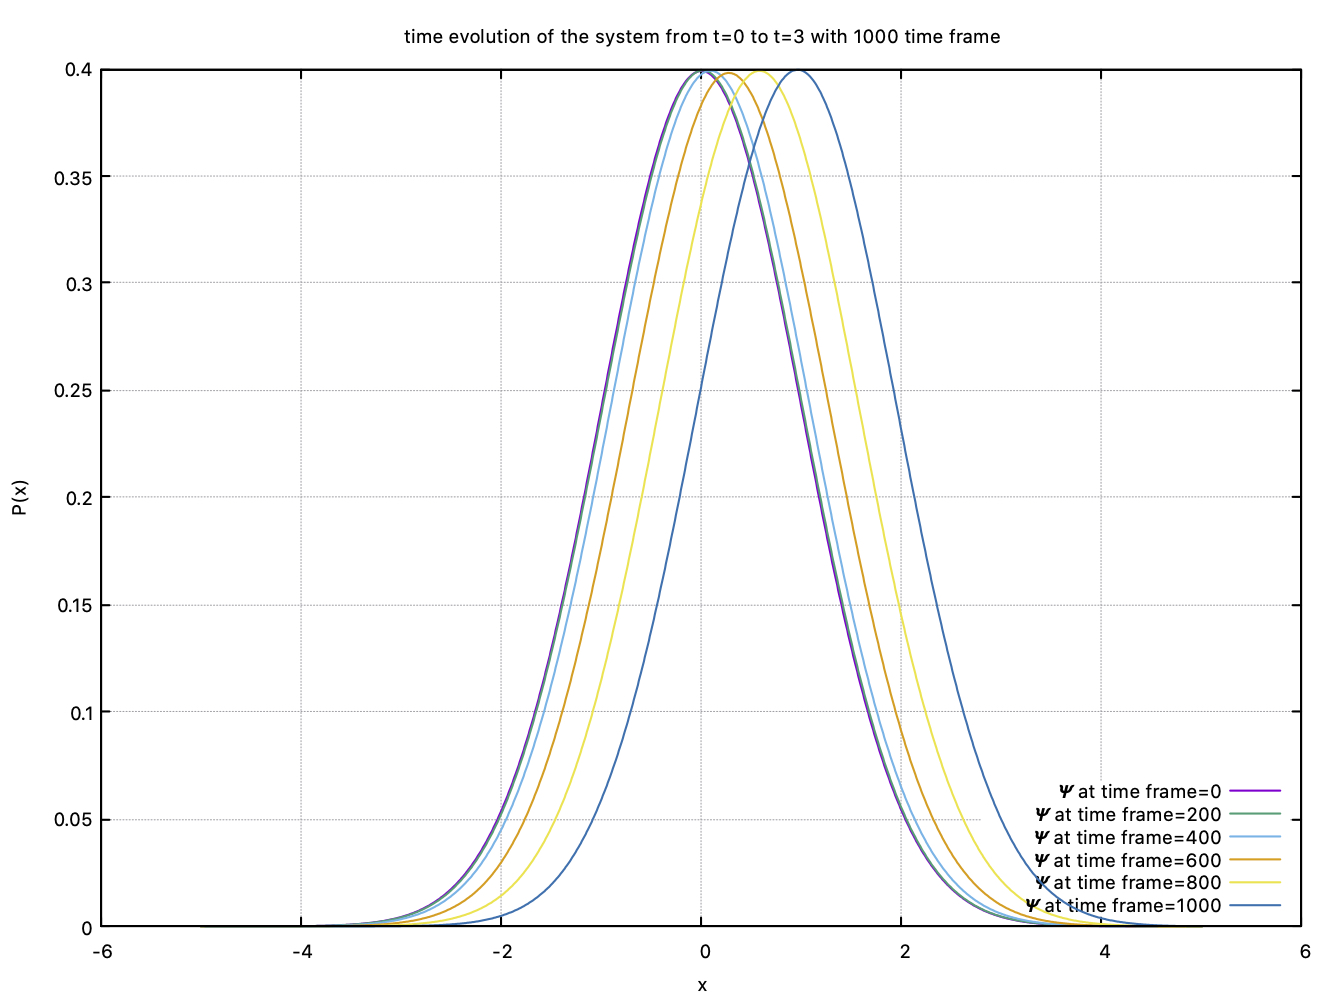
\includegraphics[width=.55\textwidth]{time_evolution}\hfill
%    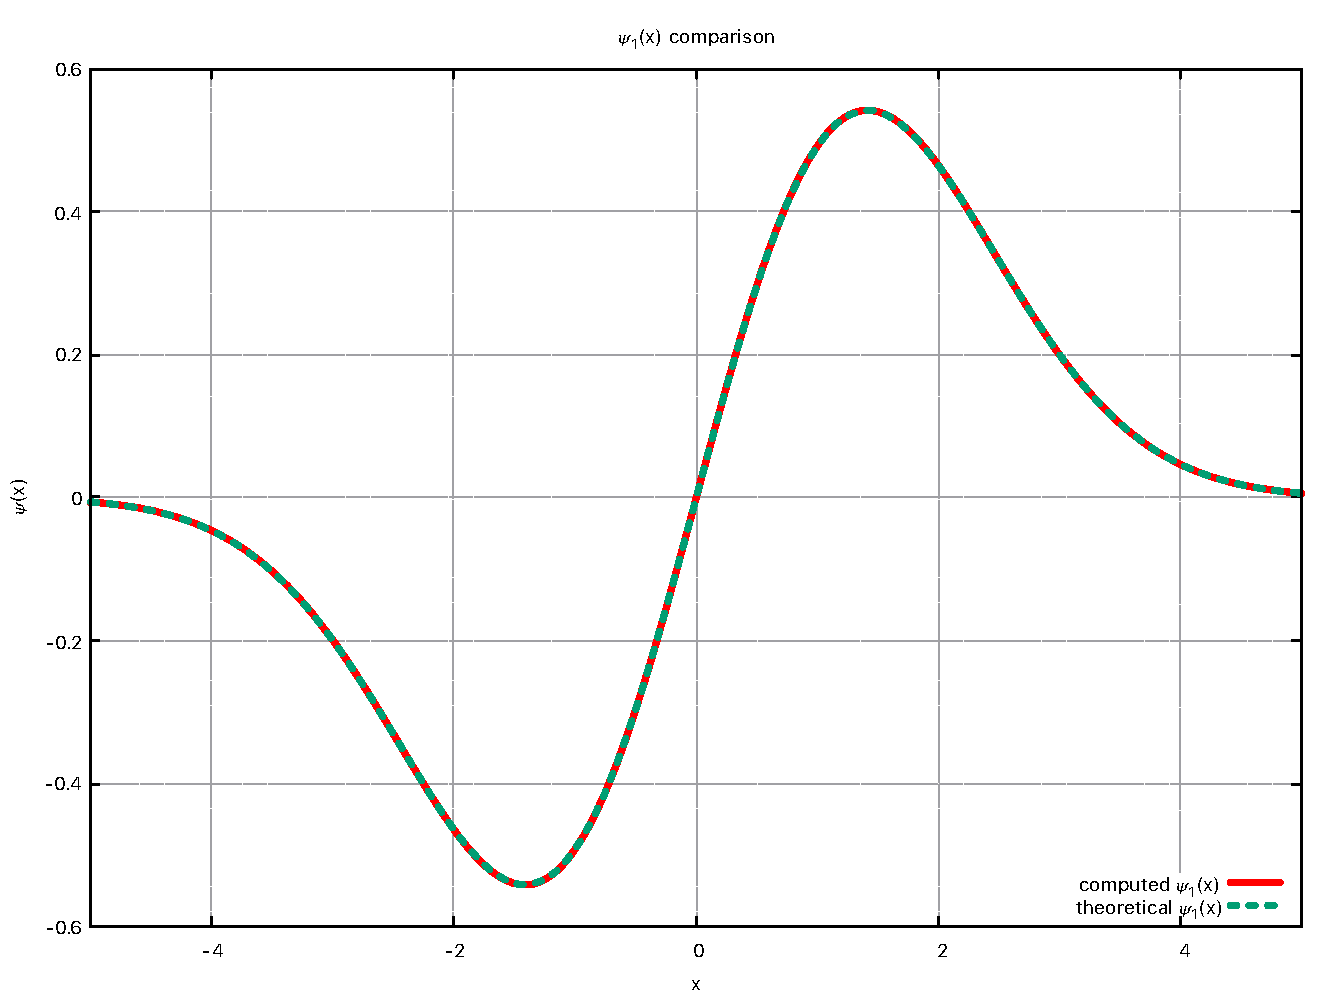
\includegraphics[width=.45\textwidth]{psi_1}\hfill
%    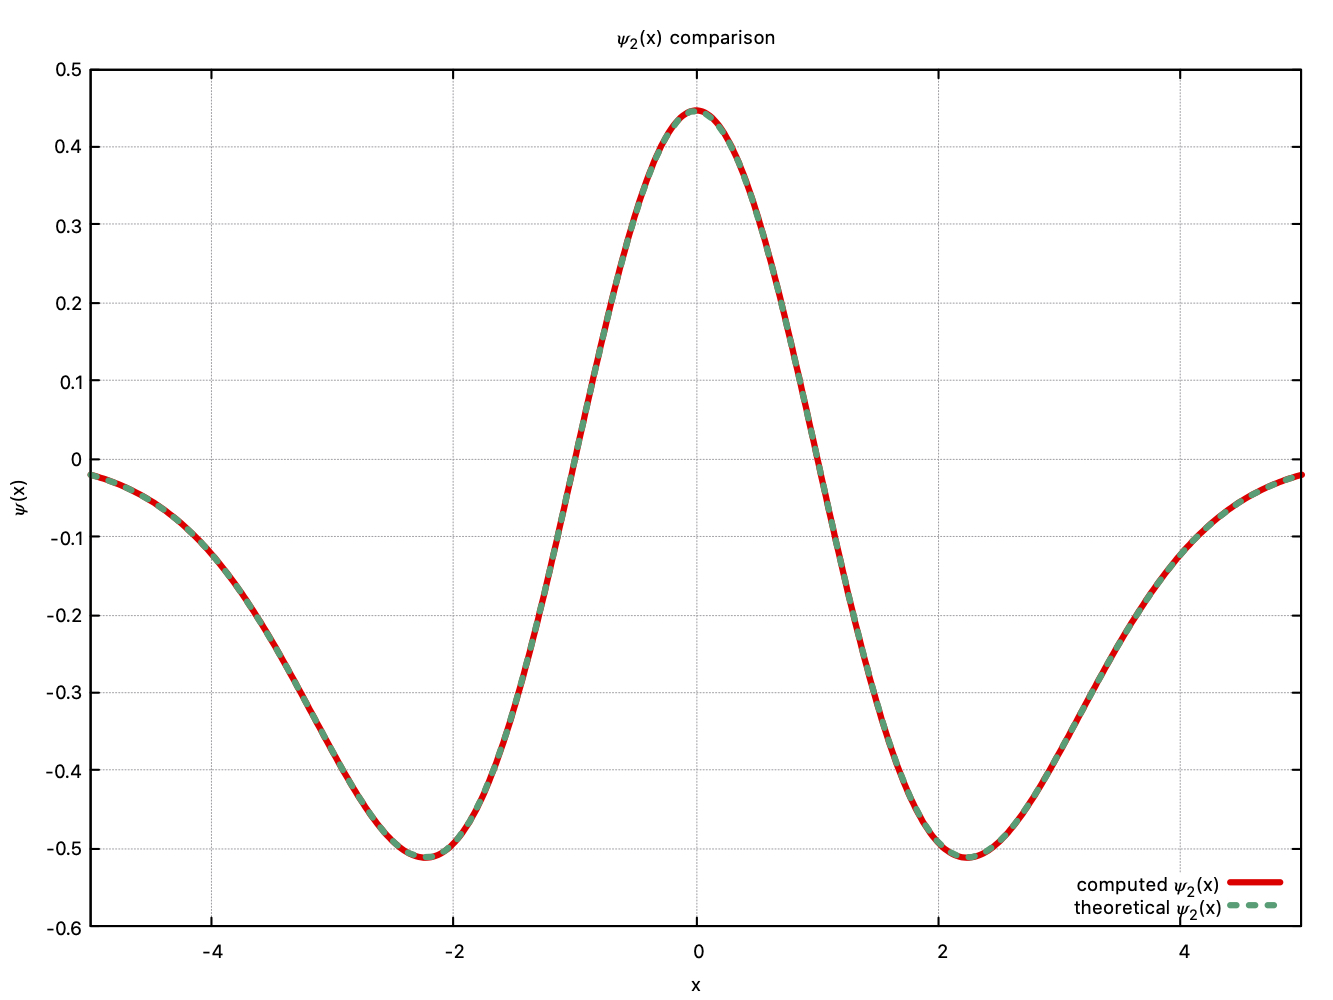
\includegraphics[width=.45\textwidth]{psi_2}
%%    \\[\smallskipamount]
%%    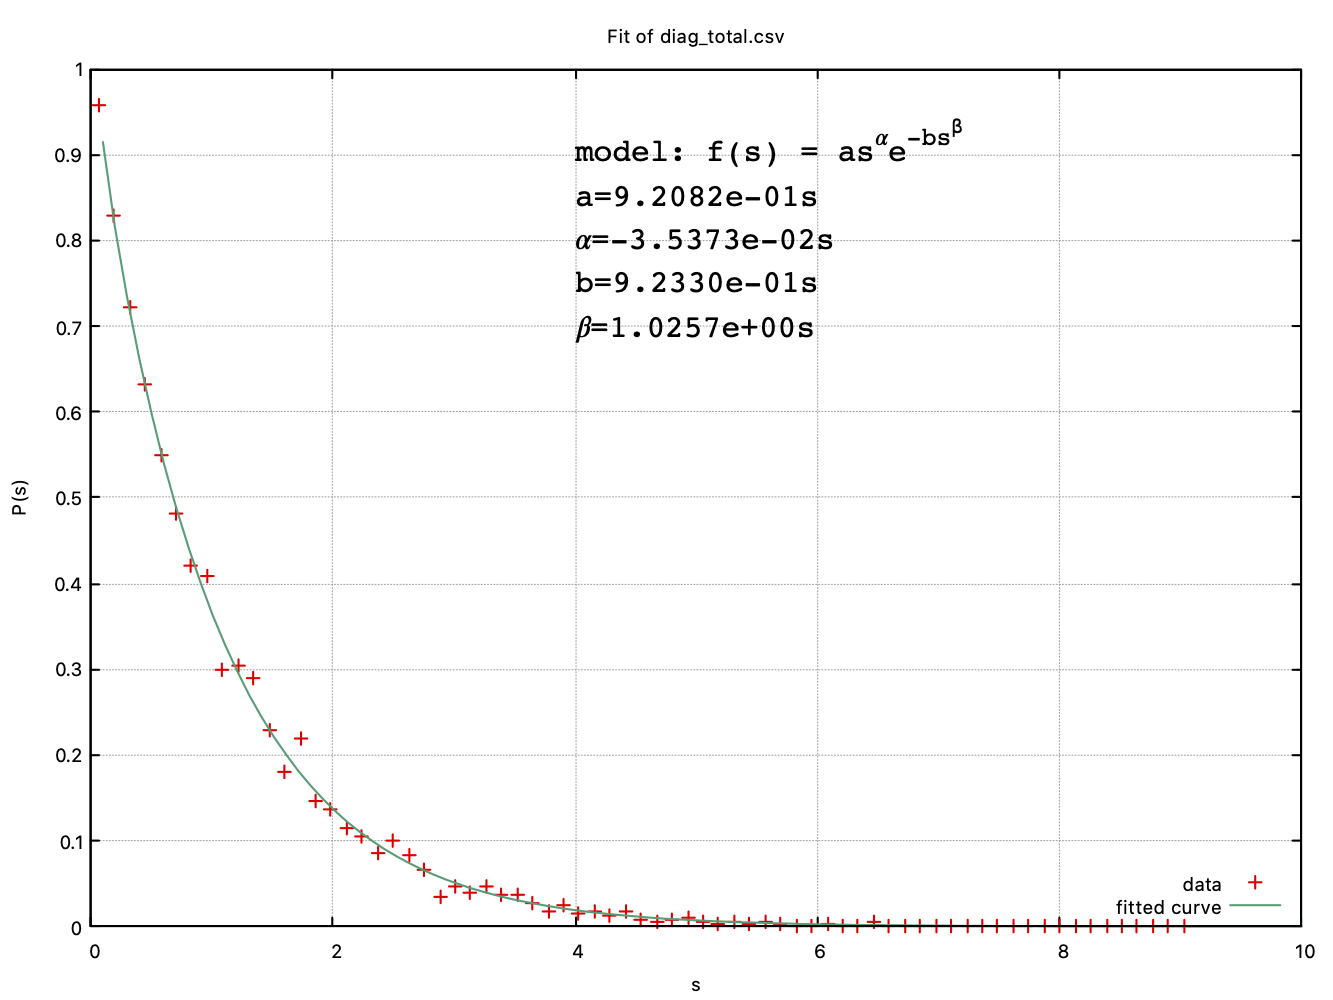
\includegraphics[width=.33\textwidth]{diag_total}\hfill
%%    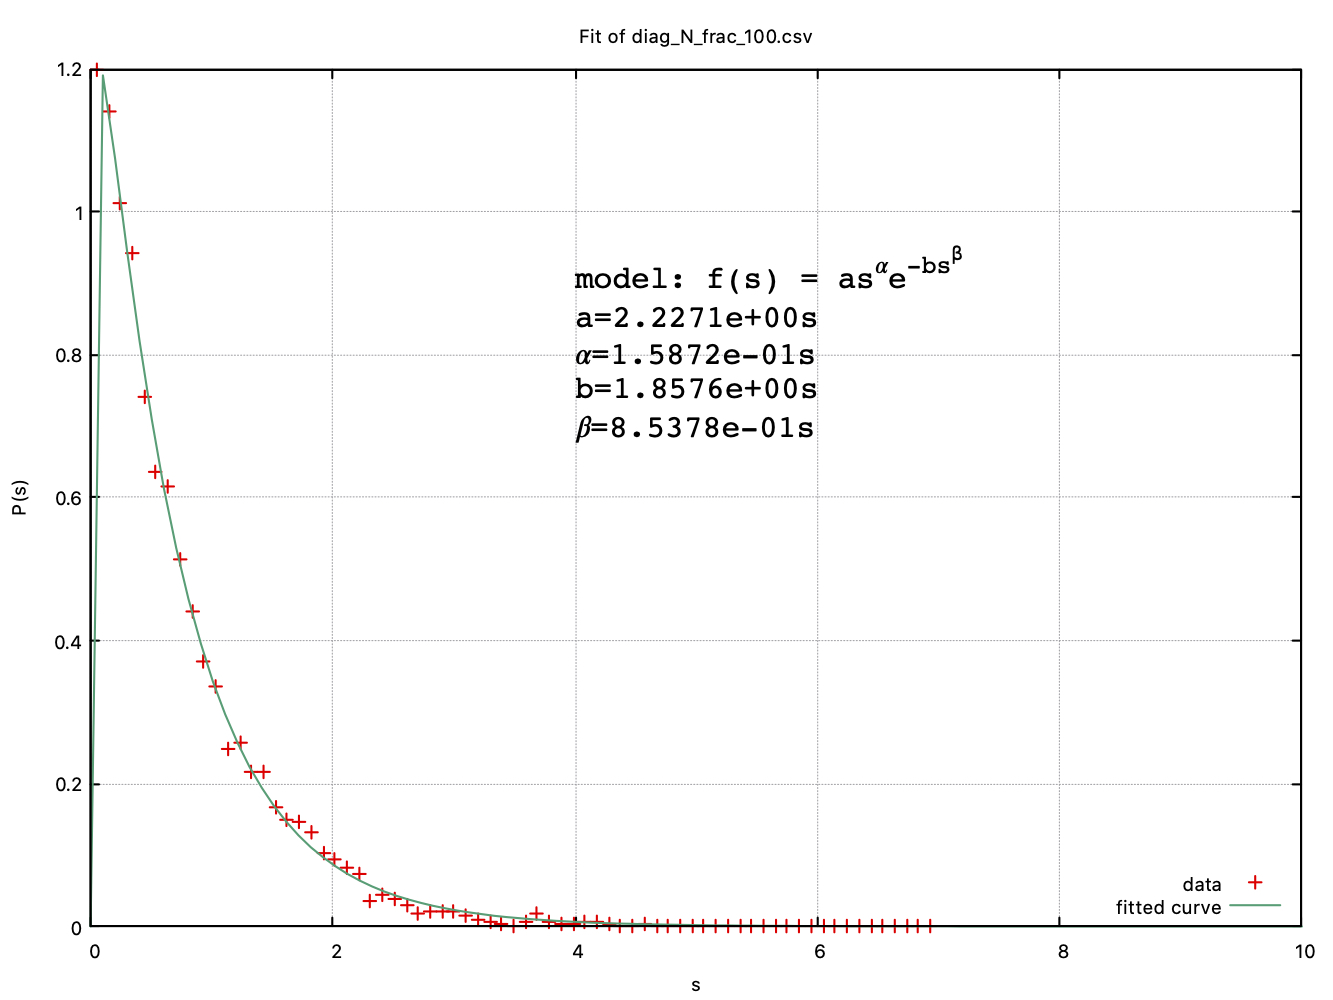
\includegraphics[width=.33\textwidth]{diag_N_frac_100}\hfill
%%    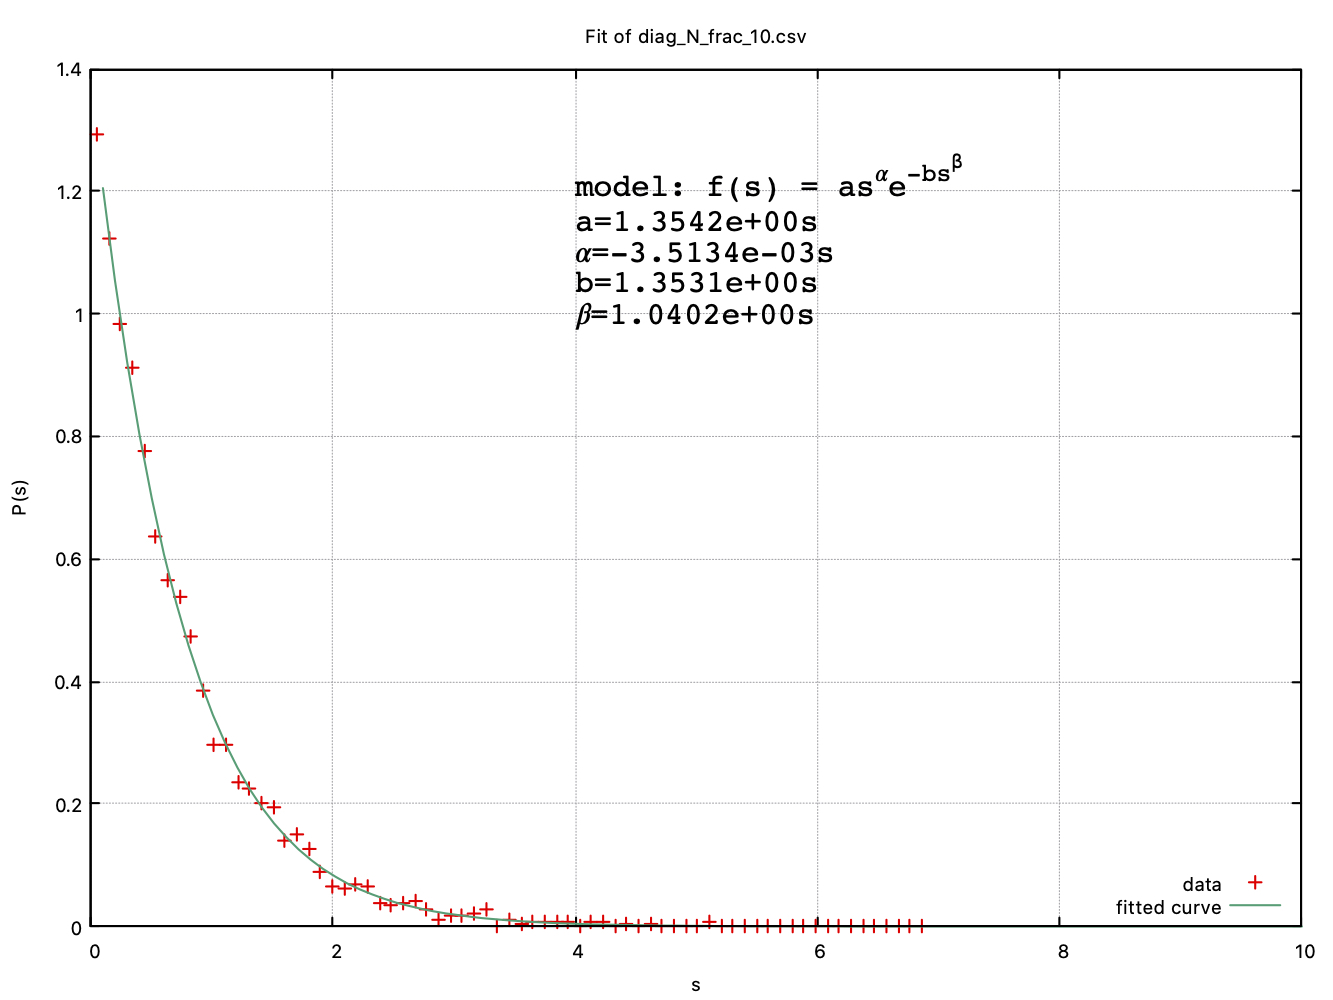
\includegraphics[width=.33\textwidth]{diag_N_frac_10}
    \caption{The system state at different time within the interval [0:3]}\label{fig:foobar}
\end{figure}

The above graph reports a result that we expected from theory. In fact the potential giver can be represented as a time-independent one in a moving reference system with costant velocity. As the time reaches $T$ we expect to have our system translated by one unit to the right.

Below I show the same graph produced for a greater time interval, and the mean position of the system during that time interval:
\begin{figure}[H]
    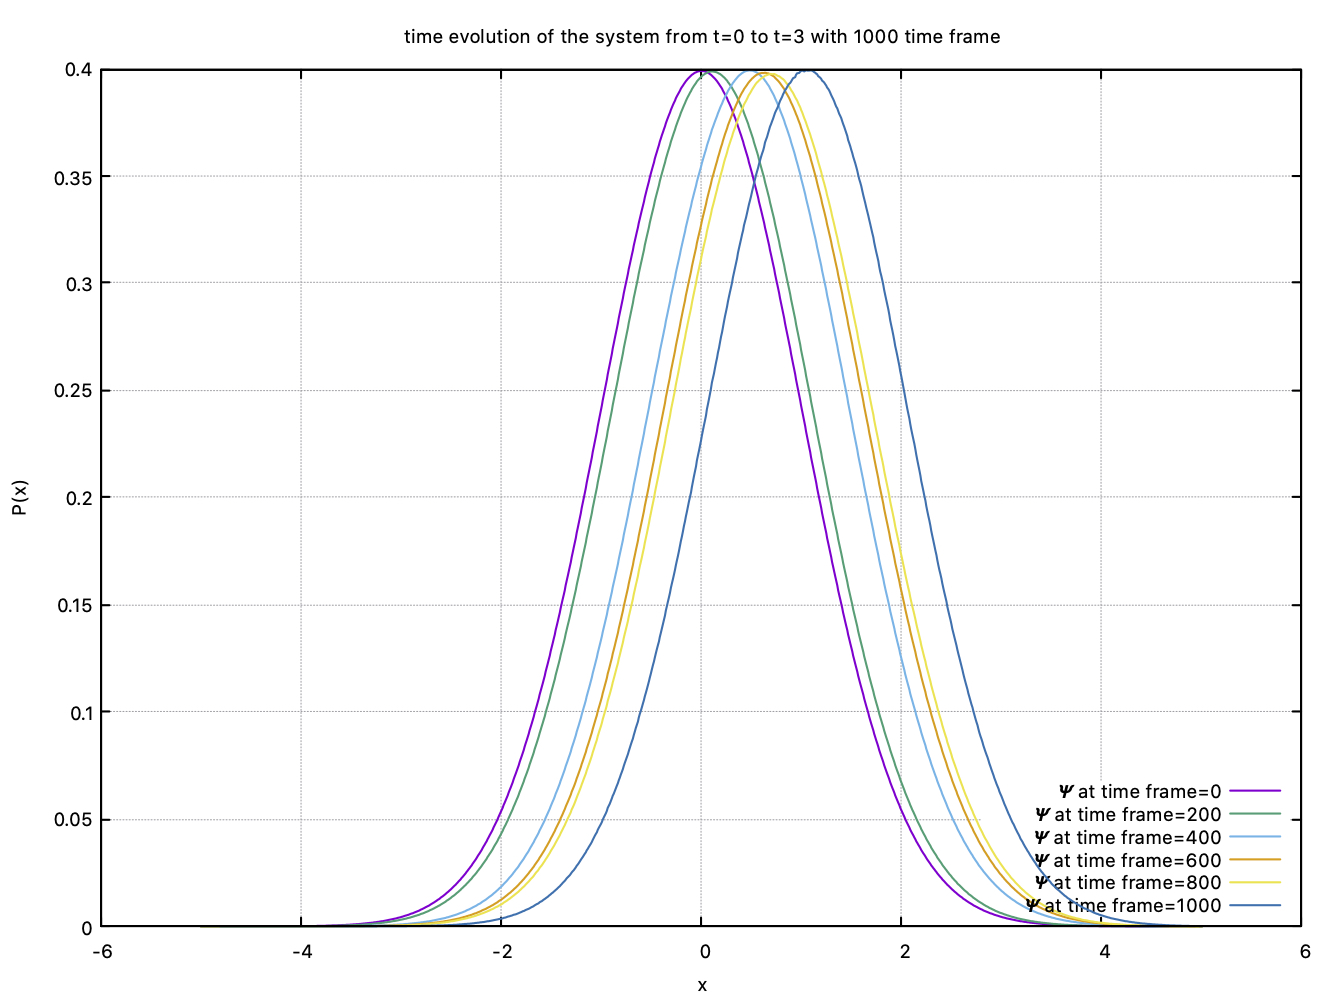
\includegraphics[width=.45\textwidth]{time_evol_10}\hfill
    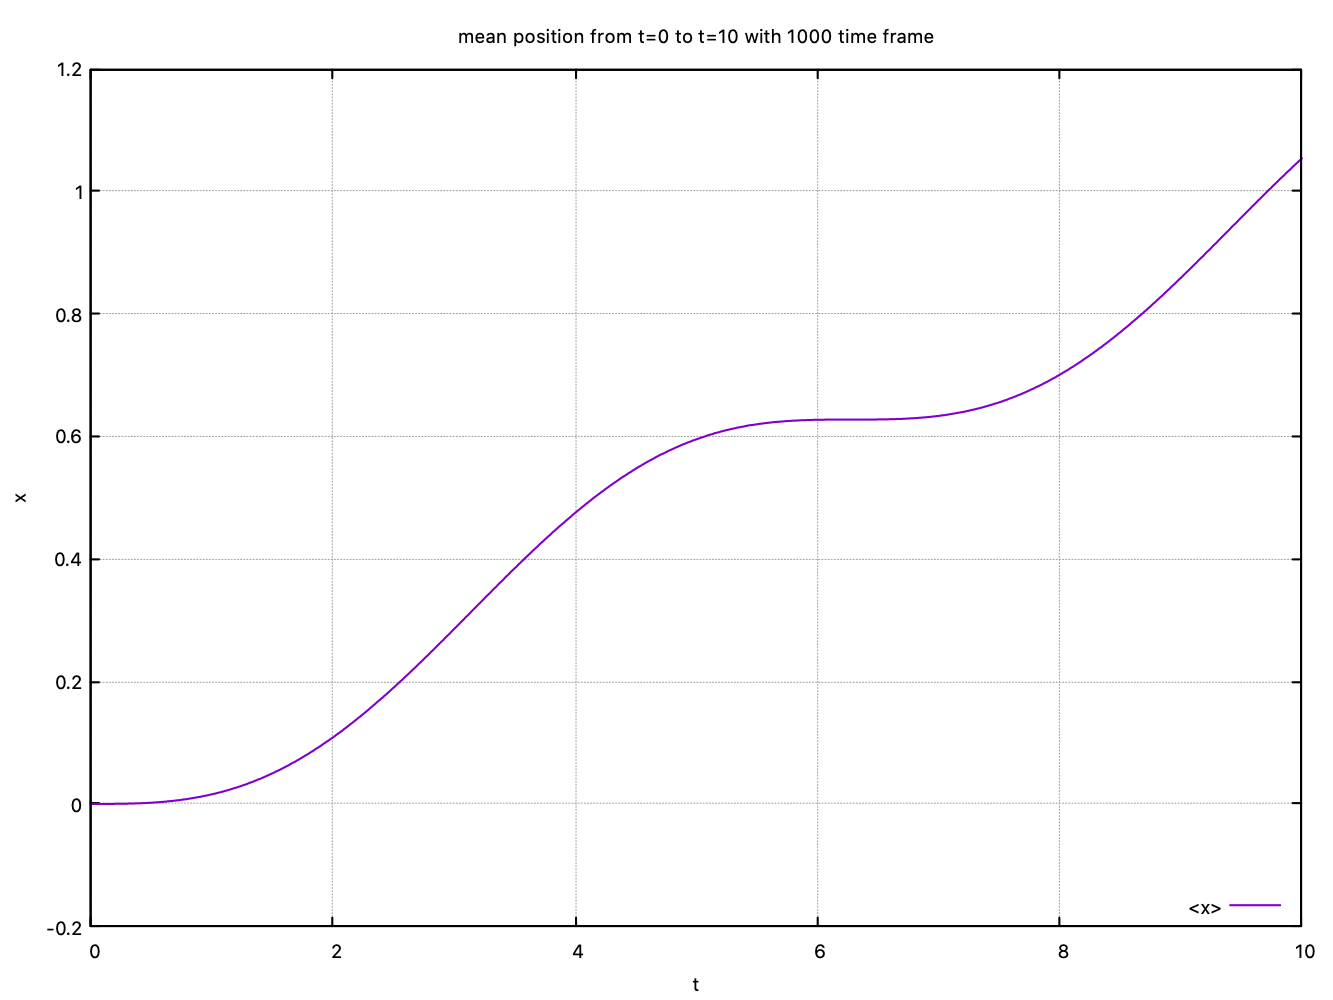
\includegraphics[width=.45\textwidth]{mean_position}\hfill
%    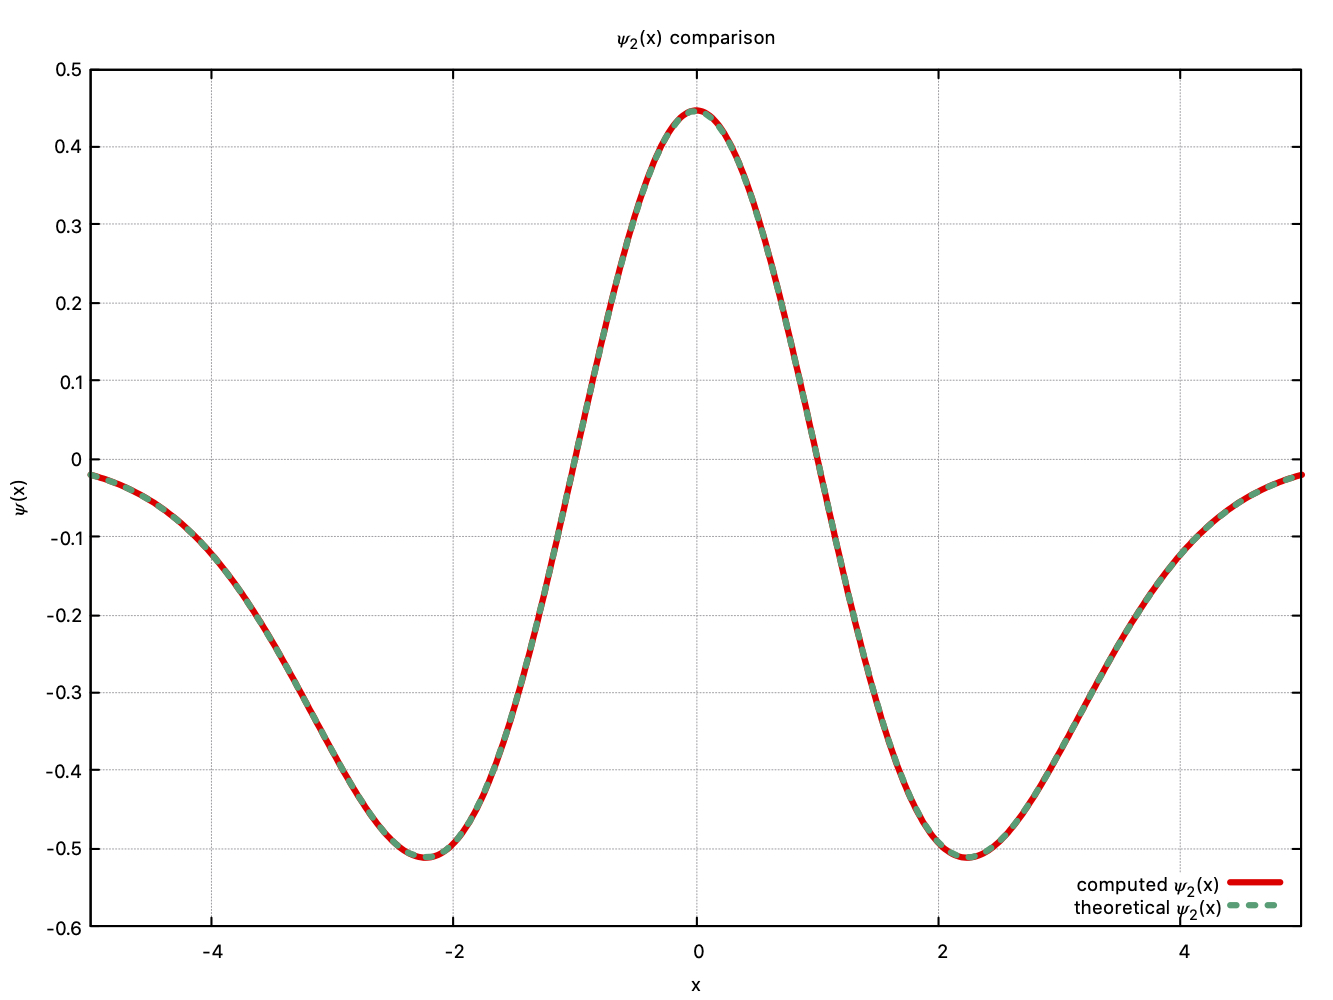
\includegraphics[width=.45\textwidth]{psi_2}
%%    \\[\smallskipamount]
%%    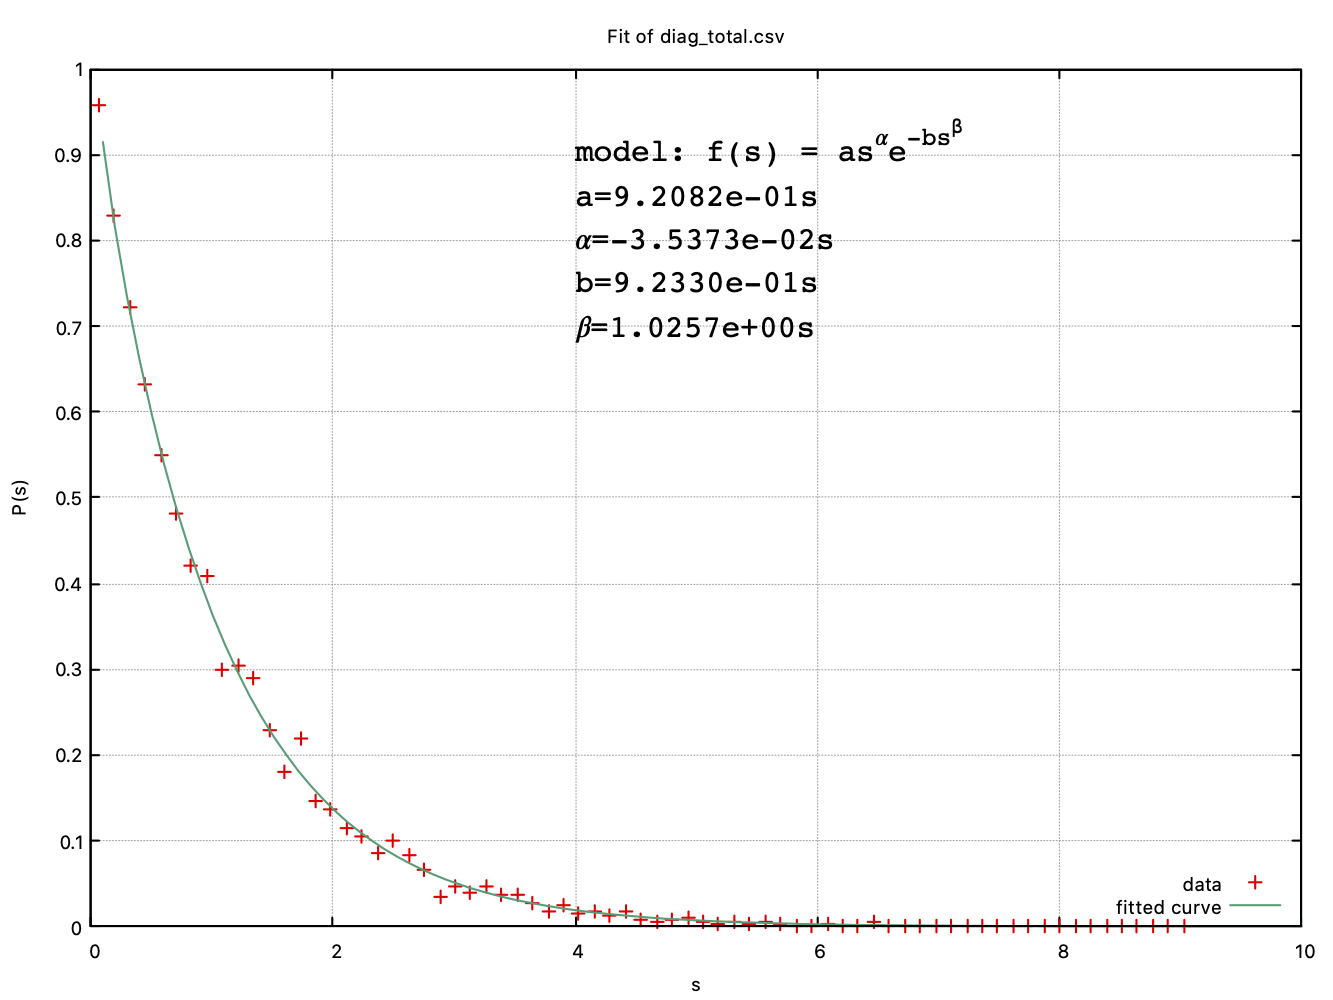
\includegraphics[width=.33\textwidth]{diag_total}\hfill
%%    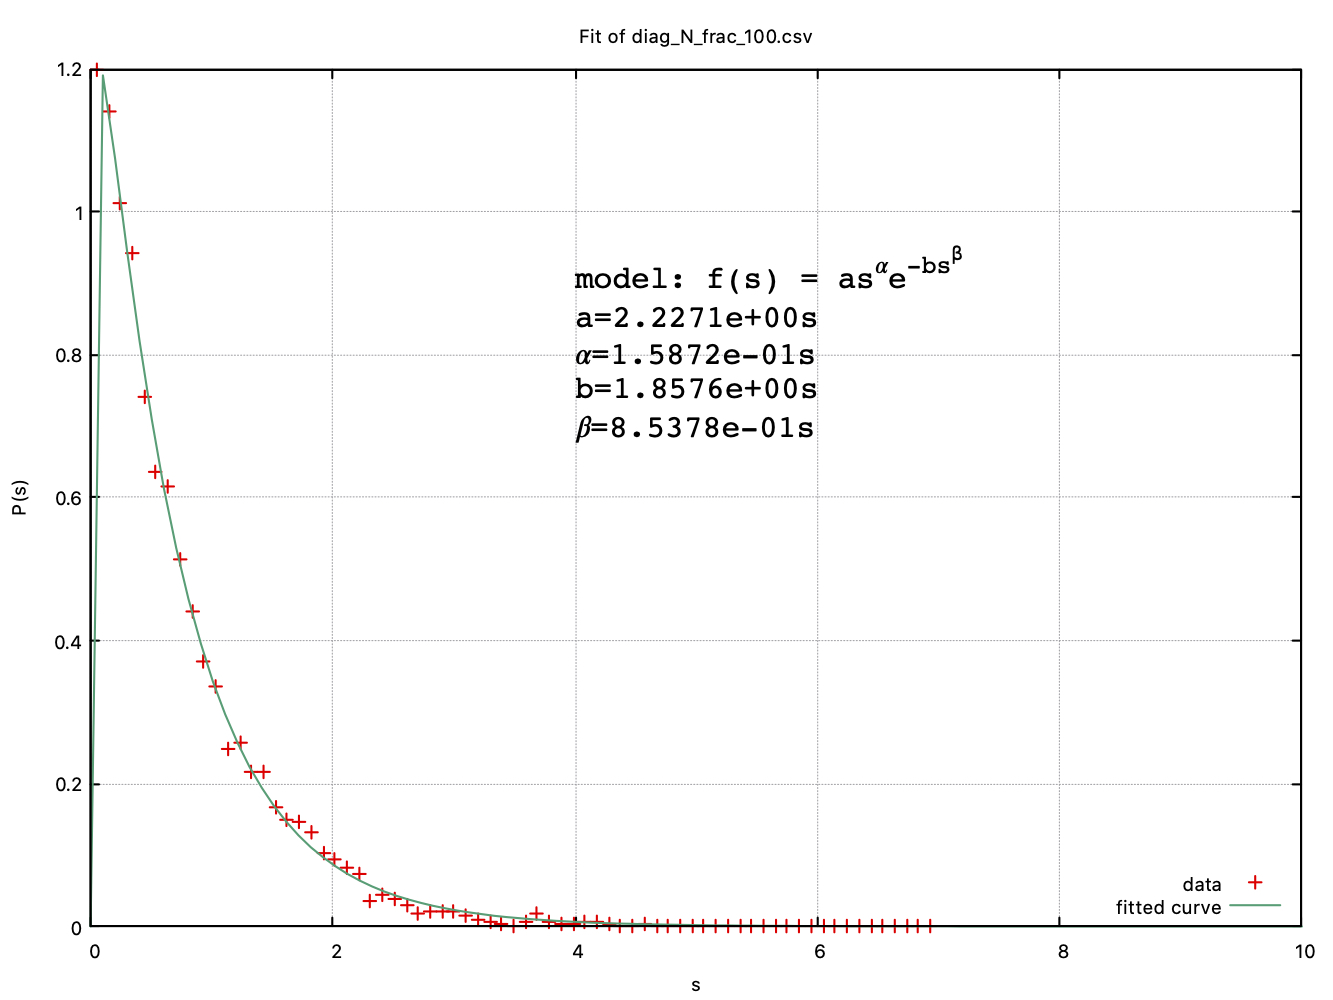
\includegraphics[width=.33\textwidth]{diag_N_frac_100}\hfill
%%    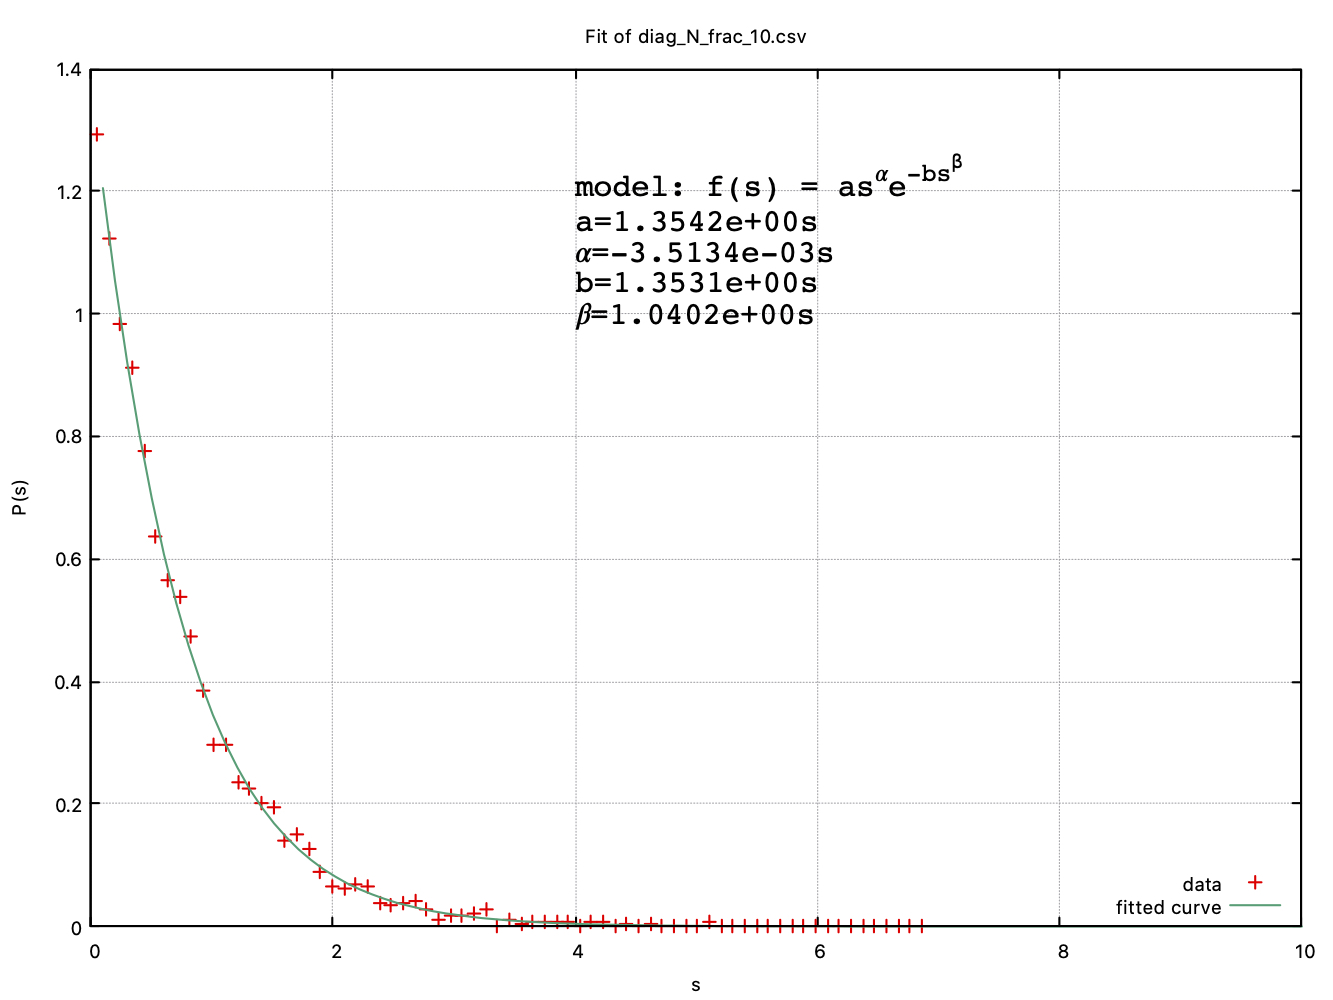
\includegraphics[width=.33\textwidth]{diag_N_frac_10}
    \caption{The system state and the mean position of the system with t varying from 0 to 10}\label{fig:foobar}
\end{figure}

\section{Self-evaluation}
I think the main objectives of the exercise are reached. I have learnt how to write a Fourier Transform through the \textit{fftw3} library and I have learnt how to implement the Split Operator Method.



\end{document}
